\section{Conclusion et perspectives}\label{sec:methodo_conclusion}

    
    Dans ce chapitre, nous avons présenté une méthodologie permettant de faciliter l'utilisation d'architectures hétérogènes dans les plateformes de calcul haute performance. Afin de motiver la réalisation de ce travail, nous avons commencé par rappeler l'importance de l'utilisation de matériels hétérogènes dans les supercalculateurs. Nous avons aussi relevé que cette hétérogénéité n'en était qu'à ses débuts avec l'utilisation des GPU. Pour répondre à ce besoin, nous avons détaillé les cinq étapes (voir \autoref{pic:methodologie_step_3}) permettant d'utiliser les outils présentés dans le chapitre précédent.
    
    \begin{figure}[h!]
    \center
    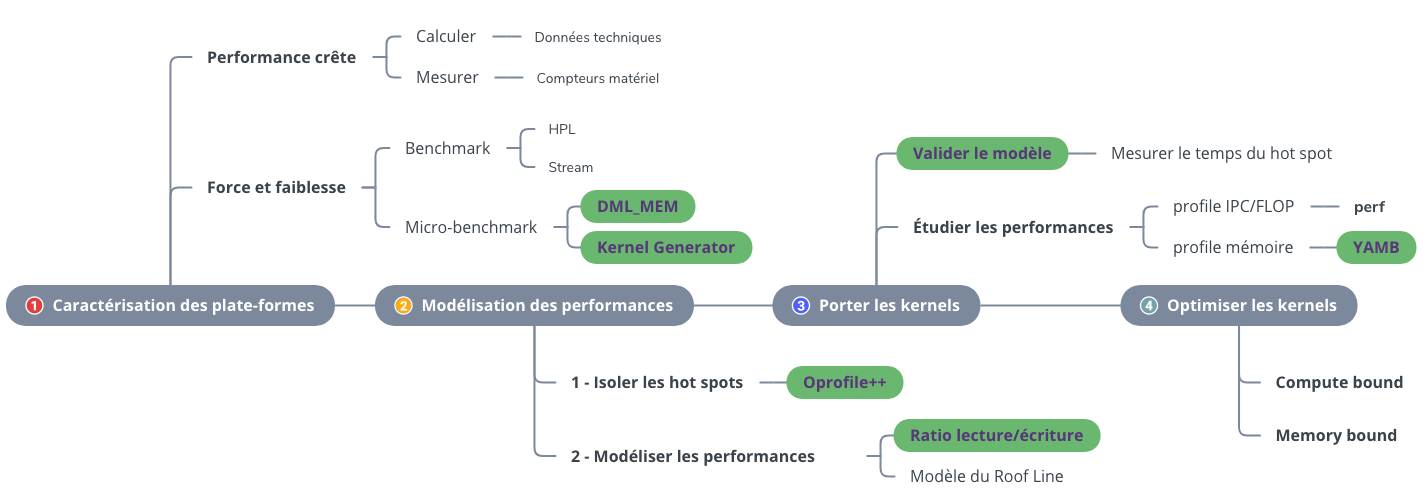
\includegraphics[width=17cm]{images/methodologie_step.png}
    \caption{\label{pic:methodologie_step_3} Méthodologie en 5 étapes pour caractériser et optimiser une application sur une nouvelle architecture.}    \end{figure}
    
    
    Dans un premier temps, nous avons discuté de la recherche et de la caractérisation de ces nouvelles plateformes. Pour cela, nous avons résumé les principales caractéristiques qu'il est nécessaire de posséder pour réaliser un premier tri. Nous avons ensuite présenté comment les outils de benchmark pouvaient être utilisés pour caractériser la performance et le comportement des microarchitectures.
    
    Dans un second temps, nous nous sommes intéressés à l'application et à la nécessité de posséder un outil permettant d'identifier ses noyaux de calculs et de modéliser leur performance. La performance de la majorité des applications de calcul haute performance étant limitée par celle du bus mémoire, nous avons présenté un modèle de performance simple, basé sur la le ratio de lecture/écriture et la taille des jeux de données. 
    
    Après avoir caractérisé les architectures et modélisé les noyaux des applications, nous avons discuté dans une quatrième étape des principaux facteurs à étudier, lors du choix d'une nouvelle architecture. La performance n'étant qu'un critère parmi d'autres tel que le coût TCO de la solution, la consommation électrique ou la difficulté des transformations nécessaires.
    
    Enfin, nous avons présenté une dernière étape permettant de valider le modèle de performance précédemment réalisé. Lorsque le code n'atteint pas les performances espérées, nous proposons un cheminement pour trouver d'où vient le problème et comment atteindre les performances souhaitées. 
    
    Pour illustrer la méthodologie, nous avons présenté pour chaque étape son application sur l'application Stream et sur un processeur Intel Skylake. Cet exercice nous permet de montrer que même pour un code aussi simple et en apparence optimisée, l'approche et les outils utilisés permettent de comprendre et d'optimiser ses performances.
    
    
    

\subsection{Perspectives}
%%%%%%%%%%%%%%%%%%%%%%%%%%%%%%%%%%%%%%%%%%%

    Lors de l'étape cinq, nous proposons un cheminement à suivre pour comprendre la mauvaise performance d'un code et des pistes à suivre pour l'améliorer. Cette étape demande une très bonne connaissance du matériel (microarchitectures, stockage, réseaux), mais aussi du logiciel (système d'exploitation, programmation à mémoire partagée et distribuée). L'expérience acquise durant ces travaux de thèse nous a montré que chaque cas était différent et qu'il fallait beaucoup d'expérience pour identifier les goulots d'étranglement et comprendre les mauvaises performances. Un travail préliminaire a été réalisé, permettant de guider l'utilisateur dans son analyse en expliquant quand utiliser chaque outil et comment transformer le code à partir des informations extraites.
    
    
    %Si certains constructeurs et utilisateurs continuent de poursuivre la stratégie visant à ajouter toujours plus de serveurs \textit{standards}, ils seront dépassés par ceux ayant commencé à investir ces nouvelles technologies plusieurs années avant eux. Il est donc crucial de s'y préparer en ayant la bonne méthodologie et les bons outils pour pouvoir profiter de ces nouvelles technologies. 

